\documentclass[10pt]{article}
\usepackage{tikz}
\usepackage{verbatim}
\newcommand{\myGlobalTransformation}[2]
{
    \pgftransformreset;
    \pgftransformcm{1.6}{0}{0.6}{0.5}{\pgfpoint{#1cm}{#2cm}}
}

\newcommand\tru{\mathrm{T}}
\newcommand\fal{\mathrm{F}}

\newcommand\ddraw[2]{
        \draw[-,line width=3pt,draw=white] (#1) -- (#2);
        \draw (#1) -- (#2);
}

\begin{document}
\pagestyle{empty}


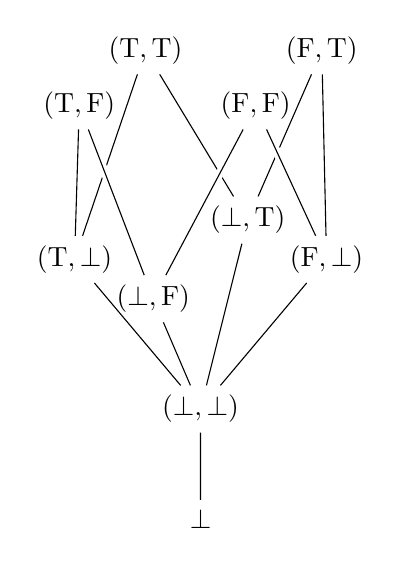
\begin{tikzpicture}

    %draws helper-grid:
%    \gridThreeD{0}{0}{black!50};
%    \gridThreeD{0}{4.25}{black!50};

    %draws lower graph lines and those in z-direction:
    \begin{scope}
        \myGlobalTransformation{0}{0.7};
        \node (bottom) at (0,0) {$\bot$};

        \myGlobalTransformation{0}{2.1};
        \node (botbot) at (0,0) {$(\bot,\bot)$};

        \myGlobalTransformation{0}{4};
        \node (trubot) at (-1,0)  {$(\tru,\bot)$};
        \node (bottru) at (0,1)  {$(\bot,\tru)$};
        \node (falbot) at (1,0) {$(\fal,\bot)$};
        \node (botfal) at (0,-1) {$(\bot,\fal)$};

        \myGlobalTransformation{0}{6.3};
        \node (trutru) at (-0.7, 0.7) {$(\tru,\tru)$};
        \node (faltru) at ( 0.7, 0.7) {$(\fal,\tru)$};
        \node (falfal) at ( 0.7,-0.7) {$(\fal,\fal)$};
        \node (trufal) at (-0.7,-0.7) {$(\tru,\fal)$};

        \draw (bottom) -- (botbot);

        \draw (botbot) -- (trubot);
        \draw (botbot) -- (bottru);
        \draw (botbot) -- (falbot);
        \draw (botbot) -- (botfal);

        \ddraw{trubot}{trutru};
        \ddraw{bottru}{trutru};
        \ddraw{falbot}{faltru};
        \ddraw{bottru}{faltru};
        \ddraw{trubot}{trufal};
        \ddraw{botfal}{trufal};
        \ddraw{botfal}{falfal};
        \ddraw{falbot}{falfal};

    \end{scope}


%
%    \begin{scope}
%        \myGlobalTransformation{0}{0};
%        \graphLinesHorizontal;
%
%        %draws all graph lines in z-direction (reset transformation first!):
%        \foreach \x in {1,3,5,7} {
%            \foreach \y in {1,3,5,7} {
%                \node (thisNode) at (\x,\y) {};
%                {
%                    \pgftransformreset
%                    \draw[white,myBG]  (thisNode) -- ++(0,5);
%                    \draw[black,very thick] (thisNode) -- ++(0,5);
%                }
%            }
%        }
%    \end{scope}
%
%    %draws upper graph-lines:
%    \begin{scope}
%        \myGlobalTransformation{0}{5};
%        \graphLinesVertical;
%    \end{scope}
%
%    % draws all graph nodes:
%    \graphThreeDnodes{0}{0};
%    \graphThreeDnodes{0}{5};
%
\end{tikzpicture}

\end{document}